\section{Partial TEST: robustness, replication and interpretation}\label{sec:resROBUST}
The analyses in this section were \emph{not} registered. They were chosen after the registered rule outcomes of Section~\ref{sec:resPARTIAL} were known, to probe the threats a sceptical reader would raise first, and they are computed by \texttt{partial/robustness.py} from the saved judged rows of the same archive with the frozen estimator code; no image was generated or re-judged. All quantities are partial-TEST and exploratory.

\paragraph{Evidence integrity.} The archive merges exactly the jobs of the present shards' manifests (Table~\ref{tab:partial-cov}); every merged image was judged once and has one DINOv2 embedding (17{,}002 each, unique identifiers), and the frozen de-duplication rules then remove 28 repeated generations. A second, independent judging of the same images on different hardware and software (one consumer GPU with PyTorch~2.6 instead of two data-centre GPUs with PyTorch~2.11) reproduced every judged outcome on all \rbRepMatched{} de-duplicated rows (\rbRepShare\%), and all four registered rule outcomes; bootstrap $p$-values differed by at most $0.002$. Two numerical warnings raised during the analysis come from scenes without an eligible pair for a constraint type and from degenerate bootstrap resamples in the HF Spearman statistic; the frozen code treats both as missing, which leaves the point estimates unchanged but makes the relative-size Spearman interval ($[-1,1]$) uninformative.

\paragraph{What CFG changes about timing (HD).} Presence persistence moves monotonically earlier with guidance: $t_{50}=\rbTwoPres$ steps at $w=2$, \rbSevenPres{} at $w=7.5$ and \rbFifteenPres{} at $w=15$ (Table~\ref{tab:partial-t50-w}, Figure~\ref{fig:partial-hd-dose}a). Two checks argue against the effect being produced by the chance correction itself. Chance agreement between independent seeds is not higher at $w=15$ ($\bar A_0=\rbAzeroFifteen$) than at $w=2$ (\rbAzeroTwo), so the correction does not favour high guidance; and the uncorrected branch--base agreement at $t=18$ is already higher at $w=15$ (\rbRawFifteen) than at $w=2$ (\rbRawTwo). The registered bootstrap resamples all \rbHdUnion{} scenes of the guidance levels, of which only \rbHdScenes{} have branches at both $w=2$ and $w=15$; resampling only those gives the same estimate with interval $[\rbHdInfLo,\rbHdInfHi]$ (Table~\ref{tab:partial-robust-hd}). The sign agrees in both TEST\_CORE shards and in four of five scene categories; in the \rbHdCountN{} counting scenes the contrast reverses (\rbHdCount{} steps), so the effect is not uniform across prompt types.

The conclusion is fragile in one specific way. Under the independent-error stress test of Eq.~\eqref{eq:err-corr} the estimate stays negative, but its interval reaches zero already at $e=0.05$ ($\rbHdFive$, $[\rbHdFiveLo,\rbHdFiveHi]$) and at $e=0.10$; at the audited presence error rate ($e=\rbErrPres$) every corrected curve exceeds $0.5$ at the first grid step, so $t_{50}$ is left-censored at all guidance scales and the contrast is not identifiable (Figure~\ref{fig:partial-hd-dose}b). The HD result therefore holds only if the presence judge's errors are mostly content-dependent rather than independent across seeds. That is plausible for a detector but is not established by our audit, which measured accuracy, not the error structure.
% generated by partial/robustness.py
\begin{table}[t]\centering\small
\caption{Commitment time by guidance scale on canonical prompts (restart D8, 40 steps; partial TEST, exploratory). $\bar A_0$: mean chance agreement of independent seeds.}\label{tab:partial-t50-w}
\begin{adjustbox}{max width=\linewidth}\begin{tabular}{rrrrr}
\toprule
$w$ & $t_{50}$ presence & 95\% CI & $\bar A_0$ presence & $t_{50}$ binding$\mid$pres. \\
\midrule
2 & 22.5 & [19.5, 27.9] & 0.729 & -- \\
7.5 & 16.2 & [12.4, 19.1] & 0.649 & 19.8 \\
15 & 13.8 & [6.9, 17.2] & 0.697 & 12.5 \\
\bottomrule
\end{tabular}\end{adjustbox}
\par\smallskip\footnotesize ``--'' marks a curve that never reaches $C = 0.5$ on the grid (right-censored, $t_{50} > 36$).
\end{table}

% generated by partial/robustness.py
\begin{table}[t]\centering\small
\caption{Robustness of the HD presence contrast $\Delta t_{50} = t_{50}(w{=}15) - t_{50}(w{=}2)$ (steps; scene-bootstrap 95\% CI). Judge-error rows correct $C(t)$ for symmetric, non-differential misclassification at rate $e$ (Eq.~\ref{eq:err-corr}); the offset row subtracts the presence offset of the DEV full-resample control from $C(t)$ at every $w$. All rows use the registered bootstrap draws; ``scenes'' counts scenes with branches at both $w = 2$ and $w = 15$. Partial TEST, exploratory.}\label{tab:partial-robust-hd}
\begin{adjustbox}{max width=\linewidth}\begin{tabular}{lrrr}
\toprule
Analysis & scenes & $\Delta t_{50}$ & 95\% CI \\
\midrule
registered estimate and interval ($e = 0$; bootstrap over all 111 scenes) & 67 & -8.67 & [-16.34, -4.72] \\
resampling only the scenes with $w = 2$ and $w = 15$ branches & 67 & -8.67 & [-16.25, -4.63] \\
judge error $e = 0.050$ & 67 & -12.91 & [-15.46, 0.71] \\
judge error $e = 0.100$ & 67 & -5.55 & [-13.41, 0.00] \\
judge error $e = 0.144$ (audit) & 67 & 0.00 & [-8.46, 0.00] \\
$C(t) - 0.159$ (DEV full-resample presence offset) & 67 & -10.96 & [-17.95, -3.83] \\
TEST\_CORE shard 0 only & 33 & -6.64 & [-15.52, 5.60] \\
TEST\_CORE shard 1 only & 34 & -9.66 & [-22.00, -5.65] \\
category: binding & 20 & -16.44 & [-24.00, -4.91] \\
category: counting & 10 & 11.40 & [9.00, 15.00] \\
category: multi & 17 & -7.71 & [-18.50, 9.67] \\
category: presence & 10 & -10.00 & [-21.00, 10.67] \\
category: spatial & 10 & -0.67 & [-12.40, 22.33] \\
\bottomrule
\end{tabular}\end{adjustbox}
\par\smallskip\footnotesize Subgroup rows have few scenes; an interval that includes 0 there is a statement about power, not about the effect.
\end{table}

\begin{figure}[t]\centering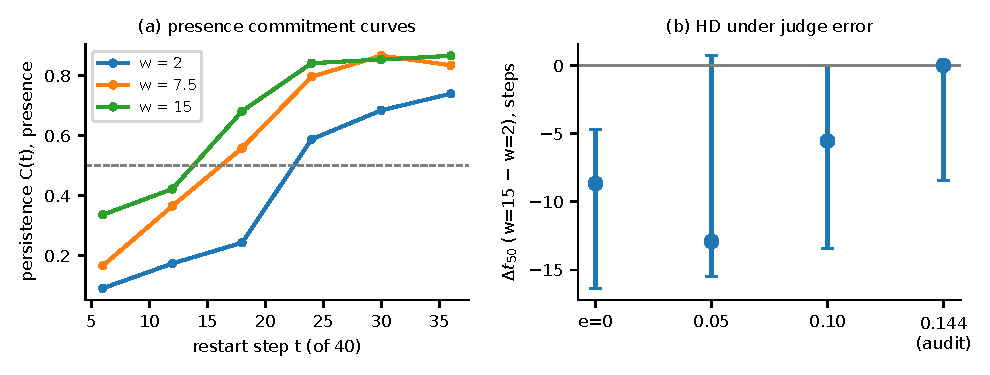
\includegraphics[width=\linewidth]{figures/partial_hd_dose.pdf}
\caption{\textbf{Partial TEST, exploratory.} (a) Presence persistence $C(t)$ at three guidance scales (restart D8, canonical prompts). (b) The HD contrast $\Delta t_{50}=t_{50}(w{=}15)-t_{50}(w{=}2)$ with 95\% scene-bootstrap intervals, without correction ($e=0$, the registered estimand) and under the independent-error stress test of Eq.~\eqref{eq:err-corr}; at the audited error rate all curves are left-censored and the contrast is $0$ by construction.}\label{fig:partial-hd-dose}\end{figure}

\paragraph{What CFG changes about adherence.} On the 102 scenes generated at every guidance level and step count, the presence rate rises from \rbRatePresTwo{} at $w=2$ to \rbRatePresFifteen{} at $w=15$ and the rate of images satisfying every constraint from \rbRateAllTwo{} to \rbRateAllFifteen{}, with most of the gain reached by $w\approx5$--$10$; halving the number of steps to 20 changes neither curve beyond its uncertainty (Figure~\ref{fig:partial-cfg-rates}). Even at the best guidance scale fewer than one image in five satisfies its whole prompt, which is the failure rate the paper set out to explain.
\begin{figure}[t]\centering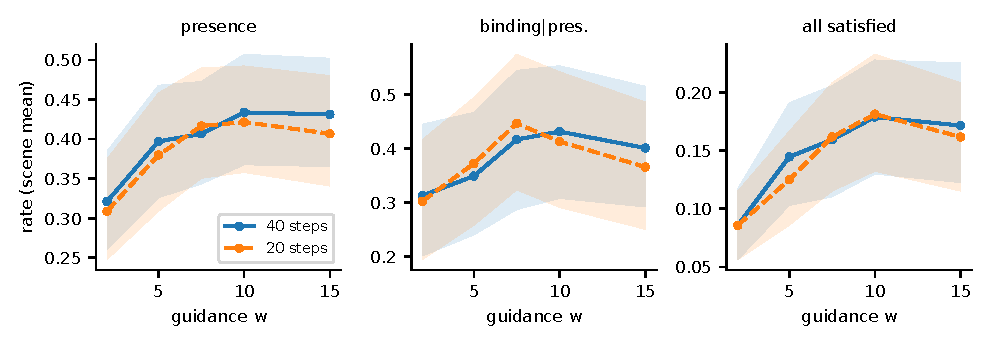
\includegraphics[width=\linewidth]{figures/partial_cfg_rates.pdf}
\caption{\textbf{Partial TEST, exploratory.} Constraint satisfaction on canonical prompts against the guidance scale (scene means over a common set of 102 scenes, 95\% scene-bootstrap bands) at 40 and 20 DDIM steps. Binding given presence is shown although its judge missed the audit criterion.}\label{fig:partial-cfg-rates}\end{figure}

\paragraph{Commitment times do not replicate from DEV to TEST.} Table~\ref{tab:dev-vs-test} compares $t_{50}$ at $w=7.5$ on the two splits. DEV placed colour binding at or before the first grid step, presence at \rbDevPres{} and count last (\rbDevCount); the partial TEST places count (\rbTestCount) and presence (\rbTestPres) before binding (\rbTestBind), and joint binding moves from \rbDevJoint{} to \rbTestJoint{}. The equal-ratio probe shows the same shift, so it is not specific to the D8 noise schedule. The DEV presence value lies outside the TEST bootstrap interval. We cannot attribute the shift: the TEST estimate covers two of three shards, DEV failed its own precision gate, and the binding judge is not validated. The shift does, however, matter for CAG: its switch steps were read off DEV ($s^\star=12$ for presence, binding and spatial prompts), and on the TEST scenes binding is not yet persistent at step 12, so A2 lowers guidance before the constraint it is meant to protect is settled.
% generated by partial/robustness.py
\begin{table}[t]\centering\small
\caption{Commitment time $t_{50}$ (steps of 40, $w = 7.5$) on DEV (the values that set $s^\star$) and on the partial TEST split. $\le6$: left-censored at the first grid step. Only presence has a validated judge. Exploratory.}\label{tab:dev-vs-test}
\begin{adjustbox}{max width=\linewidth}\begin{tabular}{lrrrr}
\toprule
Type & DEV D8 & TEST D8 & DEV ER30 & TEST ER30 \\
\midrule
presence & 9.3 & 16.2 & 9.7 & 13.3 \\
count & 18.9 & 15.3 & 15.8 & 14.0 \\
binding$\mid$presence & $\le6$ & 19.8 & $\le6$ & 21.0 \\
spatial$\mid$presence & 6.0 & $\le6$ & $\le6$ & $\le6$ \\
size$\mid$presence & -- & 13.6 & -- & -- \\
joint binding & 13.0 & 21.2 & 11.5 & 21.3 \\
scenes & 100 & 111 & 100 & 67 \\
\bottomrule
\end{tabular}\end{adjustbox}
\par\smallskip\footnotesize DEV sets the frozen switch steps $s^\star = 12$ (presence, binding, spatial prompts) and $s^\star = 21$ (count prompts).
\end{table}


\paragraph{CAG: dose, not timing (HE).} The registered HE contrast compares CAG with constant $w=7.5$, but every CAG arm applies less guidance on average ($\bar w=\rbMeanWAtwo$ for A2, A4 and A6). The dose-matched controls separate the two factors (Table~\ref{tab:partial-he-arms}, Figure~\ref{fig:partial-he-arms}). The diversity gain of A2 over A1 (+\rbDivAtwo) is matched by a constant schedule at the same mean (A6, +\rbDivAsix) and exceeded by the reversed schedule (A4, +\rbDivAfour); at equal mean guidance, A2 is \emph{less} diverse than A6 (\rbDivTwoSix, $[\rbDivTwoSixLo,\rbDivTwoSixHi]$) and A4 (\rbDivAtwoFour), and its adherence does not differ from A6 ($\Delta F=\rbFTwoSix$, $[\rbFTwoSixLo,\rbFTwoSixHi]$). The one-switch-for-all variant A3 lowers adherence ($\Delta F=\rbFAthree$, $[\rbFAthreeLo,\rbFAthreeHi]$). The pre-declared presence-only sensitivity of A2 against A1 is \rbPresAtwo{} ($[\rbPresAtwoLo,\rbPresAtwoHi]$). On these data, concentrating guidance before the DEV commitment step buys nothing that the same amount of constant guidance does not, and costs diversity relative to spending it late, in line with reports that guidance at high noise levels reduces diversity \citep{kynkaanniemi2024interval} and that late conditioning helps alignment \citep{grimal2025step}.
% generated by partial/robustness.py
\begin{table}[t]\centering\small
\caption{Guidance-schedule contrasts paired by scene (difference, 95\% CI); A1 is constant $w = 7.5$. $\bar w$: mean applied guidance of the two arms. Presence is the only judged family that met the audit criterion. Partial TEST, exploratory.}\label{tab:partial-he-arms}
\begin{adjustbox}{max width=\linewidth}\begin{tabular}{lrrlll}
\toprule
Contrast & $\bar w$ & scenes & $\Delta F$ & $\Delta$ presence & $\Delta$ diversity \\
\midrule
A2 (CAG) $-$ A1 & 4.64 vs 7.50 & 67 & -0.016 [-0.039, 0.006] & -0.026 [-0.052, 0.000] & 0.022 [0.015, 0.029]$^{\dagger}$ \\
A3 (global $s^\star$) $-$ A1 & 4.35 vs 7.50 & 67 & -0.031 [-0.056, -0.006]$^{\dagger}$ & -0.045 [-0.082, -0.015] & 0.030 [0.022, 0.038] \\
A4 (reversed) $-$ A1 & 4.64 vs 7.50 & 67 & -0.021 [-0.062, 0.017] & -0.015 [-0.063, 0.034] & 0.040 [0.016, 0.064] \\
A6 (constant at A2 mean) $-$ A1 & 4.64 vs 7.50 & 67 & -0.005 [-0.041, 0.029]$^{\dagger}$ & -0.015 [-0.063, 0.030] & 0.027 [0.009, 0.045] \\
A2 $-$ A6 (timing at equal dose) & 4.64 vs 4.64 & 134 & -0.002 [-0.026, 0.023] & -0.011 [-0.043, 0.021] & -0.013 [-0.026, -0.001] \\
A2 $-$ A4 (registered timing contrast) & 4.64 vs 4.64 & 134 & 0.001 [-0.025, 0.027]$^{\dagger}$ & -0.015 [-0.049, 0.021] & -0.030 [-0.044, -0.015] \\
\bottomrule
\end{tabular}\end{adjustbox}
\par\smallskip\footnotesize $^{\dagger}$Output of the registered analysis (its own bootstrap draws); other cells are post-hoc. ``scenes'': scenes with both arms. A1 exists only for scenes of the present TEST\_CORE shards, so contrasts with A1 use 67 scenes (all in CAG shard 1); contrasts between CAG arms use all 134.
\end{table}

\begin{figure}[t]\centering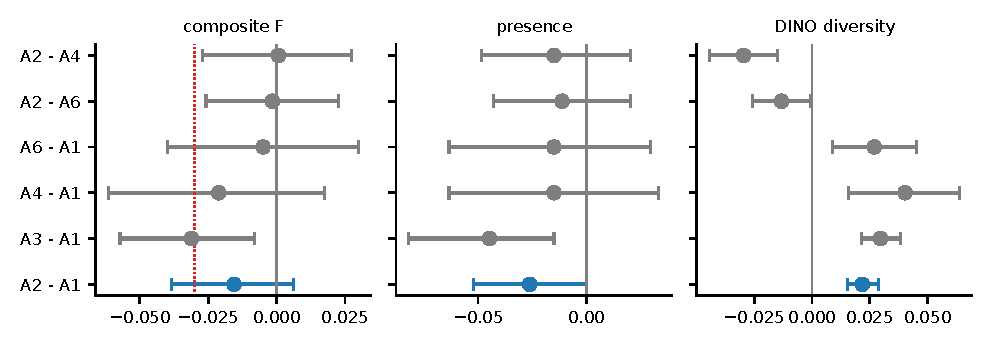
\includegraphics[width=\linewidth]{figures/partial_he_arms.pdf}
\caption{\textbf{Partial TEST, exploratory.} Paired scene-level contrasts of the guidance schedules (95\% intervals). Rows ``A$k$ $-$ A1'' compare against constant $w=7.5$ (67 scenes with both arms); ``A2 $-$ A6'' and ``A2 $-$ A4'' compare schedules with equal mean guidance (134 scenes). Dotted line: the registered non-inferiority margin $-0.03$ on $F$.}\label{fig:partial-he-arms}\end{figure}
